%------------------ vorlage.tex ------------------------------------------------
%
% LaTeX-Vorlage zur Erstellung von Projektdokumentationen
% im Fachbereich Informatik der Hochschule Trier
%
% Basis: Vorlage 'svmono' des Springer Verlags
% Bearbeiter: Hermann Schloß, Christian Bettinger
%
%-------------------------------------------------------------------------------


%------------------ Präambel ---------------------------------------------------
\documentclass[envcountsame, envcountchap, deutsch]{i-studis}

\usepackage[utf8]{inputenc}

\usepackage[a4paper]{geometry}
\usepackage[english, ngerman]{babel}

\usepackage[pdftex]{graphicx}
\usepackage{epstopdf}

\usepackage{listings}

\usepackage[german, ruled, vlined]{algorithm2e}
\usepackage{amssymb, amsfonts, amstext, amsmath}
\usepackage{array}
\usepackage[skip=10pt]{caption}
\usepackage[usenames, dvipsnames]{color}
\usepackage[pdftex, plainpages=false]{hyperref}
\usepackage{textcomp}

\usepackage{bibgerm}
\bibliographystyle{geralpha}

\usepackage{makeidx}
\usepackage{multicol}
\makeindex

\pagestyle{myheadings}
\setlength{\textheight}{1.1\textheight}

\lstset{
	basicstyle=\scriptsize\ttfamily,
	commentstyle=\scriptsize\ttfamily\color{Gray},
	identifierstyle=\scriptsize\ttfamily,
	keywordstyle=\scriptsize\ttfamily,
	stringstyle=\scriptsize\ttfamily,
	tabsize=4,
	numbers=left,
	numberstyle=\tiny,
	numberblanklines=false,
	frame=single,
	framesep=3mm,
	framexleftmargin=7mm,
	xleftmargin=10mm,
	linewidth=144mm,
	captionpos=b,
}


%------------------ Manuelle Silbentrennung ------------------------------------
\hyphenation{Ele-men-tar-ob-jek-te ab-ge-tas-tet Aus-wer-tung House-holder-Matrix Least-Squares-Al-go-ri-th-men}


%------------------ Titelseite -------------------------------------------------
\begin{document}

\title{Titel der Arbeit auf Deutsch}
\subtitle{English Title of the Thesis}

\author{Tobias Arens}

\supervisor{Titel Vorname Nachname}

\address{Ort}
\submitdate{DD.MM.YYYY}

%------------------ Projektart -------------------------------------------------
\project{Master-Abschlussarbeit}

\mytitlepage

%------------------ Vorwort, Kurzfassung, Verzeichnisse ------------------------
\frontmatter
\preface

Ein Vorwort ist nicht unbedingt nötig. Falls Sie ein Vorwort schreiben, so ist dies der Platz, um z.B. die Firma vorzustellen, in der diese Arbeit entstanden ist, oder um den Personen zu danken, die in irgendeiner Form positiv zur Entstehung dieser Arbeit beigetragen haben.

Auf keinen Fall sollten Sie im Vorwort die Aufgabenstellung näher erläutern oder vertieft auf technische Sachverhalte eingehen.
								% Vorwort (optional)
\kurzfassung

%In der Kurzfassung soll in kurzer und prägnanter Weise der wesentliche Inhalt der Arbeit beschrieben werden. Dazu zählen vor allem eine kurze Aufgabenbeschreibung, der Lösungsansatz sowie die wesentlichen Ergebnisse der Arbeit. Ein häufiger Fehler für die Kurzfassung ist, dass lediglich die Aufgabenbeschreibung (d.h. das Problem) in Kurzform vorgelegt wird. Die Kurzfassung soll aber die gesamte Arbeit widerspiegeln. Deshalb sind vor allem die erzielten Ergebnisse darzustellen. Die Kurzfassung soll etwa eine halbe bis ganze DIN-A4-Seite umfassen.

%Hinweis: Schreiben Sie die Kurzfassung am Ende der Arbeit, denn eventuell ist Ihnen beim Schreiben erst vollends klar geworden, was das Wesentliche der Arbeit ist bzw. welche Schwerpunkte Sie bei der Arbeit gesetzt haben. Andernfalls laufen Sie Gefahr, dass die Kurzfassung nicht zum Rest der Arbeit passt.

In dieser Arbeit wird das in \citetitle{gasperini:hal-03209144} vorgestellte Verfahren implementiert. Basierend auf der Matlab-Implementierung der Autoren wurde eine hinsichtlich der Benutzbarkeit und Laufzeit eine verbesserte C++Implementierung umgesetzt.
Die Laufzeit der neuen Implementierung konnte im Vergleich nahezu halbiert werden und bei gleicher Genauigkeit der berechneten Integrale.  
Diese Verbesserungen wurden mithilfe von CPU-Parallelisierungen erreicht. 
Um die Implementierung einsetzen zu können werden ein Python-Modul sowie eine Matlab-Anbindung bereitgestellt.


\kurzfassungEN

In this paper, the method described in "An analysis of the steepest descent method to efficiently compute the 3D acoustic single-layer operator in the high-frequency regime".
is implemented. Based on the Matlab implementation of the
authors, an improved C++ implementation with respect to usability and runtime was implemented. The runtime of the new implementation has been
almost halved in comparison and with the same accuracy of the calculated
integrals. In order to be able to use this in a meaningful way, a Python module as well as a
a Matlab mex-file are provided.							% Kurzfassung/Abstract
\tableofcontents										% Inhaltsverzeichnis
\listoffigures											% Abbildungsverzeichnis (optional)
\listoftables											% Tabellenverzeichnis (optional)
\lstlistoflistings										% Listings (optional)


%------------------ Kapitel ----------------------------------------------------
\mainmatter
\chapter{Einleitung und Problemstellung}

%Begonnen werden soll mit einer Einleitung zum Thema, also Hintergrund und Ziel erläutert werden.

%Weiterhin wird das vorliegende Problem diskutiert: Was ist zu lösen, warum ist es wichtig, dass man dieses Problem löst und welche Lösungsansätze gibt es bereits. Der Bezug auf vorhandene oder eben bisher fehlende Lösungen begründet auch die Intention und Bedeutung dieser Arbeit. Dies können allgemeine Gesichtspunkte sein: Man liefert einen Beitrag für ein generelles Problem oder man hat eine spezielle Systemumgebung oder ein spezielles Produkt (z.B. in einem Unternehmen), woraus sich dieses noch zu lösende Problem ergibt.
\section{Zielsetzung}

Basierend auf der Arbeit \citetitle{gasperini:hal-03209144}\cite{gasperini:hal-03209144} soll in dieser Arbeit das daraus resultierende Verfahren neu implementiert werden.
Die ursprüngliche Implementierung in Matlab funktioniert zwar, weißt aber Unzulänglichkeiten hinsichtlich der Benutzbarkeit und auch der Performanz auf.
So kann diese Lösung lediglich in Matlab verwendet werden und bietet keine Schnittstelle für Nutzer an. Des weiteren wurden keine Maßnahmen zur Optimierung der implementierten Lösung egriffen.

In dieser Arbeit sollen diese beiden Aspekte gelöst werden. Zum einen wird eine Implementierung angestrebt welche Paralellisierungstechniken verwendet um das Laufzeitverhalten zu verbessern, sowie eine API anbietet welche einfach verwendet werden kann.
Darüber hinaus soll die Benutzbarkeit mithilfe eines Matlab-Plugins und eines Python-Moduls erleichtert werden.
Wichtig dabei ist, dass die Implementierung keinen Verlust hinsichtlich der Genauigkeit der berechneten Integrale erleidet.



\section{Aufbau der Arbeit}

In Kapitel \ref{algo} dieser Arbeit wird zunächst das in \cite{gasperini:hal-03209144} entwickelte Verfahren vorgestellt und einige wesentliche Teilaspekte erläutert.
Danach werden in Kapitel \ref{desgin} die Entwurfsbedingungen erläutert und auf die konkreten Anforderungen sowie die geplante Architektur der Umsetzung eingegangen.
In \ref{plan} wird die Planung hinsichtlich der Optimierung erläutert, welche in Kapitel \ref{analysis} ausgewertet und präsentiert werden.
Im Kapitel \ref{impl} werden einige Details der Implementierung hervorgehoben, sowie die verwendeten Technologien vorgestellt.
\chapter{Weitere Kapitel}

Die Gliederung hängt natürlich vom Thema und von der Lösungsstrategie ab. Als nützliche Anhaltspunkte können die Entwicklungsstufen oder -schritte z.B. der Software-Entwicklung betrachtet werden. Nützliche Gesichtspunkte erhält und erkennt man, wenn man sich

\begin{itemize}
	\item in die Rolle des Lesers oder
	\item in die Rolle des Entwicklers, der die Arbeit z.B. fortsetzen, ergänzen oder pflegen soll,
\end{itemize}

versetzt. In der Regel wird vorausgesetzt, dass die Leser einen fachlichen Hintergrund haben - z.B. Informatik studiert haben. D.h. nur in besonderen, abgesprochenen Fällen schreibt man in populärer Sprache, so dass auch Nicht-Fachleute die Ausarbeitung prinzipiell lesen und verstehen können.

Die äußere Gestaltung der Ausarbeitung hinsichtlich Abschnittformate, Abbildungen, mathematische Formeln usw. wird in Kapitel \ref{Bausteine} kurz dargestellt.

\chapter{LaTeX-Bausteine}\label{Bausteine}

Der Text wird in bis zu drei Ebenen gegliedert:

\begin{enumerate}
	\item Kapitel (\verb|\chapter{Kapitel}|)\index{Kapitel}
	\item Abschnitte (\verb|\section{Abschnitt}|)
	\item Unterabschnitte (\verb|\subsection{Unterabschnitt}|)
\end{enumerate}

\section{Abschnitt}\index{Abschnitt}

Lorem ipsum dolor sit amet, consetetur sadipscing elitr, sed diam nonumy eirmod tempor invidunt ut labore et dolore magna aliquyam erat, sed diam voluptua \cite{Nannen:03}. At vero eos et accusam et justo duo dolores et ea rebum. Stet clita kasd gubergren, no sea takimata sanctus est Lorem ipsum dolor sit amet. Lorem ipsum dolor sit amet, consetetur sadipscing elitr, sed diam nonumy eirmod tempor invidunt ut labore et dolore magna aliquyam erat, sed diam voluptua. At vero eos et accusam et justo duo dolores et ea rebum. Stet clita kasd gubergren, no sea takimata sanctus est Lorem ipsum dolor sit amet.

\subsection{Unterabschnitt} \index{Unterabschnitt}

Lorem ipsum dolor sit amet, consetetur sadipscing elitr, sed diam nonumy eirmod tempor invidunt ut labore et dolore magna aliquyam erat, sed diam voluptua. At vero eos et accusam et justo duo dolores et ea rebum. Stet clita kasd gubergren, no sea takimata sanctus est Lorem ipsum dolor sit amet. Lorem ipsum dolor sit amet, consetetur sadipscing elitr, sed diam nonumy eirmod tempor invidunt ut labore et dolore magna aliquyam erat, sed diam voluptua. At vero eos et accusam et justo duo dolores et ea rebum. Stet clita kasd gubergren, no sea takimata sanctus est Lorem ipsum dolor sit amet.

\section{Abbildungen und Tabellen}

Abbildung\index{Abbildung} und Tabellen\index{Tabelle} werden zentriert eingefügt. Grundsätzlich sollen sie erst dann erscheinen, nach dem sie im Text angesprochen wurden (siehe Abbildung \ref{a1}). Abbildungen und Tabellen (siehe Tabelle \ref{t1}) können im Fließtext (\verb|h=here|), am Seitenanfang (\verb|t=top|), am Seitenende (\verb|b=bottom|) oder auch gesammelt auf einer nachfolgenden Seite (\verb|p=page|) oder auch ganz am Ende der Ausarbeitung erscheinen. Letzteres sollte man nur dann wählen, wenn die Bilder günstig zusammen zu betrachten sind und die Ausarbeitung nicht zu lang ($< 20$ Seiten) ist.

\begin{figure} %[hbtp]
	\centering
	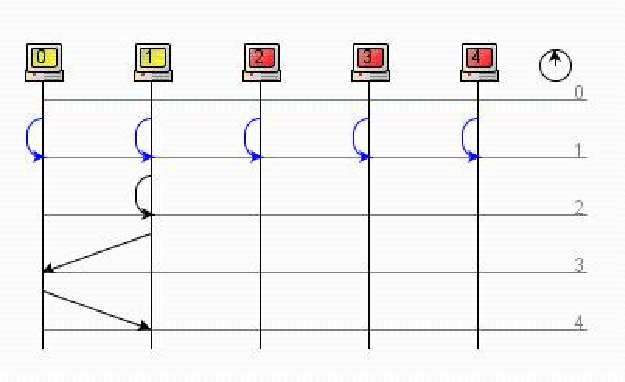
\includegraphics{images/sequence.pdf}
	\caption{Bezeichnung der Abbildung}
	\label{a1}
\end{figure}

\begin{table} %[hbtp]
	\centering
	\begin{tabular}{l | l l l l}
		\textbf{Prozesse} & \textbf{Zeit} $\rightarrow$ \\
		\hline
		$P_{1}$ & $W(x)1$ \\
		$P_{2}$ & & $W(x)2$ \\
		$P_{3}$ & & $R(x)2$ & & $R(x)1$\\
		$P_{4}$ & & & $R(x)2$ & $R(x)1$\\
	\end{tabular}
	\caption{Bezeichnung der Tabelle}
	\label{t1}
\end{table}

\section{Listings}\index{Quelltext}\index{Listing}

Lorem ipsum dolor sit amet, consetetur sadipscing elitr, sed diam nonumy eirmod tempor invidunt ut labore et dolore magna aliquyam erat, sed diam voluptua (siehe Listing \ref{quicksort.py}, Zeile 8).

\begin{lstlisting}[language=Python, caption={Quicksort-Implementierung in Python}\label{quicksort.py}]
def quicksort(arr):
less = []
pivotList = []
more = []
if len(arr) <= 1:
	return arr
else:
	pivot = arr[0]	# the pivot element
	for i in arr:
		if i < pivot:
			less.append(i)
		elif i > pivot:
			more.append(i)
		else:
			pivotList.append(i)
	less = quicksort(less)
	more = quicksort(more)
	return less + pivotList + more

print(quicksort[4, 65, 2, -31, 0, 99, 83, 782, 1]))
\end{lstlisting}

Lorem ipsum dolor sit amet, consetetur sadipscing elitr, sed diam nonumy eirmod tempor invidunt ut labore et dolore magna aliquyam erat, sed diam voluptua (siehe Listing \ref{quicksort.js}, Zeilen 3 und 5).

\begin{lstlisting}[caption={Quicksort-Implementierung in JavaScript}\label{quicksort.js}]
function quicksort([pivot, ...others]) {
	return pivot === undefined ? [] : [
		...quicksort(others.filter(n => n < pivot)),
		pivot,
		...quicksort(others.filter(n => n >= pivot))
	];
}

console.log(quicksort([11.8, 14.1, 21.3, 8.5, 16.7, 5.7]));
\end{lstlisting}

Größere Code-Fragmente sollten im Anhang eingefügt werden. \cite{wiki:listing}

\section{Mathematische Formel}\index{Formel}

Mathematische Formeln bzw. Formulierungen können sowohl im Fließtext (z.B. $y=x^2$) oder abgesetzt und zentriert im Text erscheinen. Gleichungen sollten für Referenzierungen nummeriert werden (siehe Formel \ref{gl-1}).

\begin{equation}
	\label{gl-1}
	e_{i}=\sum _{i=1}^{n}w_{i}x_{i}
\end{equation}

Entscheidungsformel:

\begin{equation}
	\psi(t)=\left\{\begin{array}{ccc}
		1 & \qquad 0 <= t < \frac{1}{2} \\
		-1 & \qquad \frac{1}{2} <= t <1 \\
		0 & \qquad sonst
	\end{array} \right.
\end{equation}

Matrix:\index{Matrix}

\begin{equation}
A = \left(
	\begin{array}{llll}
		a_{11} & a_{12} & \ldots & a_{1n} \\
		a_{21} & a_{22} & \ldots & a_{2n} \\
		\vdots & \vdots & \ddots & \vdots \\
		a_{n1} & a_{n2} & \ldots & a_{nn} \\
	\end{array}
\right)
\end{equation}

Vektor:\index{Vektor}

\begin{equation}
	\overline{a} = \left(
		\begin{array}{c}
			a_{1}\\
			a_{2}\\
			\vdots\\
			a_{n}\\
		\end{array}
	\right)
\end{equation}

\section{Sätze, Lemmata, Definitionen, Beweise, Beispiele}\index{Satz}\index{Lemma}\index{Definition}\index{Beweis}\index{Beispiel}

Sätze, Lemmata, Definitionen, Beweise und Beispiele können in speziell dafür vorgesehenen Umgebungen erstellt werden.

\begin{definition}(Optimierungsproblem)
Ein \emph{Optimierungsproblem} $\mathcal{P}$ ist festgelegt durch ein Tupel $(I_\mathcal{P}, sol_\mathcal{P}, m_\mathcal{P}, goal)$ wobei gilt

\begin{enumerate}
	\item $I_\mathcal{P}$ ist die Menge der Instanzen,
	\item $sol_\mathcal{P} : I_\mathcal{P} \longmapsto \mathbb{P}(S_\mathcal{P})$ ist eine Funktion, die jeder Instanz $x \in I_\mathcal{P}$ eine Menge zulässiger Lösungen zuweist,
	\item $m_\mathcal{P} : I_\mathcal{P} \times S_\mathcal{P} \longmapsto \mathbb{N}$ ist eine Funktion, die jedem Paar $(x,y(x))$ mit $x \in I_\mathcal{P}$ und $y(x) \in sol_\mathcal{P}(x)$ eine Zahl $m_\mathcal{P}(x,y(x)) \in \mathbb{N}$ zuordnet (= Maß für die Lösung $y(x)$ der Instanz $x$), und
	\item $goal \in \{min,max\}$.
\end{enumerate}
\end{definition}

\begin{example}
	MINIMUM TRAVELING SALESMAN (MIN-TSP)
	\begin{itemize}
		\item $I_{MIN-TSP} =_{def}$ s.o., ebenso $S_{MIN-TSP}$
		\item $sol_{MIN-TSP}(m,D) =_{def} S_{MIN-TSP} \cap \mathbb{N}^m$
		\item $m_{MIN-TSP}((m,D),(c_1, \ldots , c_m)) =_{def} \sum_{i=1}^{m-1} D(c_i, c_{i+1}) + D(c_m,c_1)$
		\item $goal_{MIN-TSP} =_{def} min$
	\end{itemize}
	\begin{flushright}$\qed$\end{flushright}
\end{example}

\begin{theorem}
Sei $\mathcal{P}$ ein \textbf{NP}-hartes Optimierungsproblem. Wenn $\mathcal{P} \in$ \textbf{PO}, dann ist \textbf{P} = \textbf{NP}.
\end{theorem}

\begin{proof}
Um zu zeigen, dass \textbf{P} = \textbf{NP} gilt, genügt es wegen Satz A.30 zu zeigen, dass ein einziges \textbf{NP}-vollständiges Problem in \textbf{P} liegt. Sei also $\mathcal{P}'$ ein beliebiges \textbf{NP}-vollständiges Problem.

Weil $\mathcal{P}$ nach Voraussetzung \textbf{NP}-hart ist, gilt insbesondere $\mathcal{P}' \leq_T \mathcal{P}_C$. Sei $R$ der zugehörige Polynomialzeit-Algorithmus dieser Turing-Reduktion. Weiter ist $\mathcal{P} \in$ \textbf{PO} vorausgesetzt, etwa vermöge eines Polynomialzeit-Algorithmus $A$. Aus den beiden Polynomialzeit-Algorithmen $R$ und $A$ erhält man nun leicht einen effizienten Algorithmus für $\mathcal{P}'$: Ersetzt man in $R$ das Orakel durch $A$, ergibt dies insgesamt eine polynomielle Laufzeit.

%\begin{flushright}$\qed$% \end{flushright}
\end{proof}

\begin{lemma}
Aus \textbf{PO} $=$ \textbf{NPO} folgt \textbf{P} $=$ \textbf{NP}.
\end{lemma}

\begin{proof}
Es genügt zu zeigen, dass unter der angegeben Voraussetzung KNAPSACK $\in$ \textbf{P} ist.

Nach Voraussetung ist MAXIMUM KNAPSACK $\in$ \textbf{PO}, d.h. die Berechnung von $m^*(x)$ für jede Instanz $x$ ist in Polynomialzeit möglich. Um KNAPSACK bei Eingabe $(x,k)$ zu entscheiden, müssen wir nur noch $m^*(x) \geq k$ prüfen. Ist das der Fall, geben wir $1$, sonst $0$ aus. Dies bleibt insgesamt ein Polynomialzeit-Algorithmus.

\begin{flushright}$\qed$\end{flushright}
\end{proof}

\section{Fußnoten}

In einer Fußnote können ergänzende Informationen\footnote{Informationen die für die Arbeit zweitrangig sind, jedoch für den Leser interessant sein könnten.} angegeben werden. Außerdem kann eine Fußnote auch Links enthalten. Wird in der Arbeit eine Software (zum Beispiel Java\footnote{\url{https://www.oracle.com/java/technologies/}}) eingesetzt, so kann die Quelle, die diese Software zur Verfügung stellt in der Fußnote angegeben werden.

\section{Literaturverweise}\index{Literatur}\index{Quellen}

Alle benutzte Literatur wird im Literaturverzeichnis angegeben\footnote{Dazu wird eine sogenannte BibTeX-Datei (literatur.bib) verwendet.}. Alle angegebene Literatur sollte mindestens einmal im Text referenziert werden \cite{Cormen:90}.

\chapter{Beispiel-Kapitel}

In diesem Kapitel wird beschrieben, warum es unterschiedliche Konsistenzmodelle\index{Konsistenzmodelle} gibt. Außerdem werden die Unterschiede zwischen strengen Konsistenzmodellen\index{Linearisierbarkeit} (Linearisierbarkeit, sequentielle Konsistenz)\index{Konsistenz!sequentiell} und schwachen Konsistenzmodellen\index{Konsistenz!schwach} (schwache Konsistenz, Freigabekonsistenz)\index{Freigabekonsistenz} erläutert. Es wird geklärt, was Strenge und Kosten (billig, teuer) in Zusammenhang mit Konsistenzmodellen bedeuten.

\section{Warum existieren unterschiedliche Konsistenzmodelle?}

Laut \cite{Malte:97} sind mit der\index{Replikation} Replikation von Daten immer zwei gegensätzliche Ziele verbunden: die Erhöhung der\index{Verfügbarkeit} Verfügbarkeit und die Sicherung der\index{Konsistenz} Konsistenz der Daten. Die Form der Konsistenzsicherung bestimmt dabei, inwiefern das eine Kriterium erfüllt und das andere dementsprechend nicht erfüllt ist (Trade-off zwischen Verfügbarkeit und der Konsistenz der Daten). Stark konsistente Daten sind stabil, das heißt, falls mehrere Kopien der Daten existieren, dürfen keine Abweichungen auftreten. Die Verfügbarkeit der Daten ist hier jedoch stark eingeschränkt. Je schwächer die Konsistenz wird, desto mehr Abweichungen können zwischen verschiedenen Kopien einer Datei auftreten, wobei die Konsistenz nur an bestimmten Synchronisationspunkten gewährleistet wird. Dafür steigt aber die Verfügbarkeit der Daten, weil sie sich leichter replizieren lassen.

Nach \cite{Mosberger:93} kann die Performanzsteigerung der schwächeren Konsistenzmodelle wegen der Optimierung\index{Optimierung} (Pufferung, Code-Scheduling, Pipelines) 10-40 Prozent betragen. Wenn man bedenkt, dass mit der Nutzung der vorhandenen Synchronisierungsmechanismen schwächere Konsistenzmodelle den Anforderungen der strengen Konsistenz genügen, stellt sich der höhere programmiertechnischer Aufwand bei der Implementierung der schwächeren Konsistenzmodelle als ihr einziges Manko dar.

In \cite{Cheriton:85} ist beschrieben, wie man sich Formen von DSM vorstellen könnte, für die ein beachtliches Maß an\index{Inkonsistenz} Inkonsistenz akzeptabel wäre. Beispielsweise könnte DSM verwendet werden, um die Auslastung von Computern in einem Netzwerk zu speichern, so dass Clients für die Ausführung ihrer Applikationen die am wenigsten ausgelasteten Computer auswählen können. Weil die Informationen dieser Art innerhalb kürzester Zeit ungenau werden können (und durch die Verwendung der veralteten Daten keine großen Nachteile entstehen können), wäre es vergebliche Mühe, sie ständig für alle Computer im System konsistent zu halten \cite{Coulouris:02}. Die meisten Applikationen stellen jedoch strengere Konsistenzanforderungen.

\section{Klassifizierung eines Konsistenzmodells}

Die zentrale Frage, die für die Klassifizierung\index{Konsistenz!streng}\index{Konsistenz!schwach} (streng oder schwach) eines Konsistenzmodells von Bedeutung ist \cite{Coulouris:02}: wenn ein Lesezugriff auf eine Speicherposition erfolgt, welche Werte von Schreibzugriffen auf diese Position sollen dann dem Lesevorgang bereitgestellt werden? Die Antwort für das schwächste Konsistenzmodell lautet: von jedem Schreibvorgang, der vor dem Lesen erfolgt ist, oder in der "`nahen"' Zukunft, innerhalb des definierten Betrachtungsraums, erfolgten wird. Also irgendein Wert, der vor oder nach dem Lesen geschrieben wurde.

Für das strengste Konsistenzmodell, Linearisierbarkeit (atomic consistency), stehen alle geschriebenen Werte allen Prozessoren sofort zur Verfügung: eine Lese-Operation gibt den aktuellsten Wert zurück, der geschrieben wurde, bevor das Lesen stattfand. Diese Definition ist aber in zweierlei Hinsicht problematisch. Erstens treten weder Schreib- noch Lese-Operationen zu genau einem Zeitpunkt auf, deshalb ist die Bedeutung von "`aktuellsten"' nicht immer klar. Zweitens ist es nicht immer möglich, genau festzustellen, ob ein Ereignis vor einem anderen stattgefunden hat, da es Begrenzungen dafür gibt, wie genau Uhren in einem verteilten System synchronisiert werden können.

Nachfolgend werden einige Konsistenzmodelle absteigend nach ihrer Strenge vorgestellt. Zuvor müssen wir allerdings klären, wie die Lese- und Schreibe-Operationen in dieser Ausarbeitung dargestellt werden.

Sei $x$ eine Speicherposition, dann können Instanzen dieser Operationen wie folgt ausgedrückt werden:

\begin{itemize}
	\item $R(x)a$ - eine Lese-Operation\index{Operation!Lesen}, die den Wert $a$ von der Position $x$ liest.
	\item $W(x)b$ - eine Schreib-Operation\index{Operation!Schreiben}, die den Wert $b$ an der Position $x$ speichert.
\end{itemize}

\section{Linearisierbarkeit\index{Linearisierbarkeit} (atomic consistency)}

Die Linearisierbarkeit im Zusammenhang mit DSM kann wie folgt definiert werden:

\begin{itemize}
	\item Die verzahnte Operationsabfolge findet so statt: wenn $R(x)a$ in der Folge vorkommt, dann ist die letzte Schreib-Operation, die vor ihr in der verzahnten Abfolge auftritt, $W(x)a$, oder es tritt keine Schreib-Operation vor ihr auf und $a$ ist der Anfangswert von $x$. Das bedeutet, dass eine Variable nur durch eine Schreib-Operation geändert werden kann.
	\item Die Reihenfolge der Operationen in der Verzahnung ist konsistent zu den \underline{Echtzeiten}\index{Echtzeiten}, zu denen die Operationen bei der tatsächlichen Ausführung aufgetreten sind.
\end{itemize}

Die Bedeutung dieser Definition kann an folgendem Beispiel (Tabelle \ref{tab:1}) nachvollzogen werden. Es sei angenommen, dass alle Werte mit $0$ vorinitialisiert sind.

\begin{table}
	\centering
		\begin{tabular}{l | l l l l}
			\textbf{Prozesse} & \textbf{Zeit} $\rightarrow$ & \\
			\hline
			$P_{1}$ & $W(x)1$ & & $W(y)2$ \\
			$P_{2}$ & & $R(x)1$ & & $R(y)2$ \\
		\end{tabular}
	\caption{Linearisierbarkeit ist erfüllt}
	\label{tab:1}
\end{table}

Hier sind beide Bedingungen erfüllt, da die Lese-Operationen den zuletzt geschriebenen Wert zurückliefern. Interessanter ist es, zu sehen, wann die Linearisierbarkeit verletzt ist.

\begin{table}
	\centering
		\begin{tabular}{l | l l l l}
		\textbf{Prozesse} & \textbf{Zeit} $\rightarrow$ \\
		\hline
		$P_{1}$ & $W(x)1$ & $W(x)2$ \\
		$P_{2}$ & & & \color{red} $R(x)0$ & \color{black} $R(x)2$ \\
		\end{tabular}
	\caption{Linearisierbarkeit ist verletzt, sequentielle Konsistenz ist erfüllt.}
	\label{tab:2}
\end{table}

In diesem Beispiel (Tabelle \ref{tab:2}) ist die Echtzeit-Anforderung verletzt, da der Prozess $P_{2}$ immer noch den alten Wert liest, obwohl er von Prozess $P_{1}$ bereits geändert wurde. Diese Ausführung wäre aber sequentiell konsistent (siehe kommender Abschnitt), da es eine Verzahnung der Operationen gibt, die diese Werte liefern könnte ($R(x)0$, $W(x)1$, $W(x)2$, $R(y)2$). Würde man beide Lese-Operationen des 2. Prozesses vertauschen, wie in der Tabelle \ref{tab:3} dargestellt, so wäre keine sinnvolle Verzahnung mehr möglich.

\begin{table}
	\centering
		\begin{tabular}{l | l l l l}
		\textbf{Prozesse} & \textbf{Zeit} $\rightarrow$ \\
		\hline
		$P_{1}$ & $W(x)1$ & $W(x)2$ \\
		$P_{2}$ & & & \color{red} $R(x)2$ & \color{red} $R(x)0$ \\

		\end{tabular}
	\caption{Linearisierbarkeit und sequentielle Konsistenz sind verletzt.}
	\label{tab:3}
\end{table}

In diesem Beispiel sind beide Bedingungen verletzt. Selbst wenn die Echtzeit, zu der die Operationen stattgefunden haben, ignoriert wird, gibt es keine Verzahnung einzelner Operationen, die der Definition entsprechen würde.

\chapter{Zusammenfassung und Ausblick}

In diesem Kapitel soll die Arbeit noch einmal kurz zusammengefasst werden. Insbesondere sollen die wesentlichen Ergebnisse Ihrer Arbeit herausgehoben werden. Erfahrungen, die z.B. Benutzer mit der Mensch-Maschine-Schnittstelle gemacht haben oder Ergebnisse von Leistungsmessungen sollen an dieser Stelle präsentiert werden. Sie können in diesem Kapitel auch die Ergebnisse oder das Arbeitsumfeld Ihrer Arbeit kritisch bewerten. Wünschenswerte Erweiterungen sollen als Hinweise auf weiterführende Arbeiten erwähnt werden.



%------------------ Literaturverzeichnis & Index -------------------------------
\backmatter
\bibliography{literatur}								% Literaturverzeichnis (literatur.bib)
\printindex												% Index (optional)


%------------------ Anhänge ----------------------------------------------------
\begin{appendix}
	\chapter{Glossar}

\abbreviation{DisASTer}		{Distributed Algorithms Simulation Terrain, eine Plattform zur Implementierung verteilter Algorithmen \cite{Gottwald:03}}

\abbreviation{DSM}			{Distributed Shared Memory}

\abbreviation{AC}			{Atomic Consistency (dt.: Linearisierbarkeit)}
\abbreviation{RC}			{Release Consistency (dt.: Freigabekonsistenz)}
\abbreviation{SC}			{Sequential Consistency (dt.: Sequentielle Konsistenz)}
\abbreviation{WC}			{Weak Consistency (dt.: Schwache Konsistenz)}
							% Glossar (optional)
	\chapter{Selbstständigkeitserklärung}

\begin{description}

\item[$\Box$] Diese Arbeit habe ich selbstständig verfasst und keine anderen als die angegebenen Quellen und Hilfsmittel verwendet.\\

\item[$\Box$] Diese Arbeit wurde als Gruppenarbeit angefertigt. Meinen Anteil habe ich selbstständig verfasst und keine anderen als die angegebenen Quellen und Hilfsmittel verwendet.\\

Namen der Mitverfasser:
\vspace{3cm}

Meine eigene Leistung ist:
\vspace{3cm}

\end{description}

\vspace{3cm}

\begin{minipage}[t]{3cm}
	\rule{3cm}{0.5pt}
	Datum
\end{minipage}
\hfill
\begin{minipage}[t]{9cm}
	\rule{9cm}{0.5pt}
	Unterschrift der Kandidatin/des Kandidaten
\end{minipage}
	% Selbstständigkeitserklärung
\end{appendix}


\end{document}
